\documentclass[aps,prd,twocolumn,superscriptaddress,nofootinbib,floatfix]{revtex4-2}

\usepackage{amsmath,amssymb,amsfonts,amsthm}
\usepackage{graphicx}
\usepackage{hyperref}
\usepackage{braket}
\usepackage{booktabs}
\usepackage{xcolor}
\usepackage{float}
\usepackage{tikz}

\newtheorem{definition}{Definition}
\newtheorem{proposition}{Proposition}
\newtheorem{theorem}{Theorem}

\graphicspath{{../../figures/}}

% Shortcuts
\newcommand{\Sig}{\Sigma}
\newcommand{\Fint}{F_{\mathrm{int}}}
\newcommand{\Fwp}{F_{\mathrm{wp}}}
\newcommand{\Tab}{T_{AB}}
\newcommand{\Gll}{G_{\lambda\lambda}}
\newcommand{\CR}{Coherence Relativity}

\begin{document}

\title{Coherence Relativity I: Coherence Frames, Frame Invariance, and the Born Rule}

\author{Bryan Kaufman}
\affiliation{Independent Researcher}
\email{bryankaufman@mac.com}

\date{\today}

\pacs{03.65.Ta, 03.67.-a, 04.60.-m}

\keywords{Quantum measurement problem, Born rule, Coherence frames, Information geometry, Fubini-Study metric, Frame invariance}

% ============================================================
% ABSTRACT
% ============================================================
\begin{abstract}
We propose that the quantum measurement problem is a frame problem, resolved by recognizing that coherence is relative to a choice of coherence frame---analogous to the relativity of simultaneity in special relativity. We introduce coherence relativity, a geometric framework in which physical reality is described on a joint manifold $\mathcal{M} \times \Sig$, where $\mathcal{M}$ is emergent spacetime and $\Sig$ is a coherence manifold whose points represent distinct observational perspectives. In this framework, wave function collapse is not a dynamical process but a transformation between coherence frames induced by measurement interactions. We present a derivation of the Born rule---that measurement probabilities equal squared amplitudes---as the unique probability measure invariant under coherence-frame relabelings and splittings, given additivity and continuity. This derivation unifies insights from Gleason's theorem, Zurek's envariance, and operational reconstruction programs within a single geometric structure. We demonstrate the framework with the double-slit experiment in two coherence frames and identify six experimentally testable signatures distinguishing \CR{} from standard quantum mechanics: non-linear visibility scaling, frame-transformation hysteresis, coherence-space curvature effects, modified gravitational decoherence, measurable transformation timescales, and coherence revival. The most accessible predictions---erasure hysteresis and transformation timescales---are testable with current superconducting qubit and trapped ion platforms.
\end{abstract}

\maketitle

% ============================================================
% SECTION 1: INTRODUCTION
% ============================================================
\section{Introduction}\label{sec:intro}

\subsection{The Measurement Problem as a Frame Problem}

The quantum measurement problem---how definite outcomes emerge from superposed states---has persisted for nearly a century despite the extraordinary empirical success of quantum mechanics. At its core lies a conceptual asymmetry: the formalism describes systems evolving unitarily, yet observations yield definite results governed by the Born rule, $p_k = |c_k|^2$. The standard resolution appends a measurement postulate that operates outside the unitary framework, creating what Penrose called ``the most important open problem in physics'' and what Bell termed ``the shifty split'' between quantum and classical domains.

Attempts to resolve this tension have proceeded along several lines. Gleason's theorem~\cite{gleasonMeasuresClosedSubspaces1957} showed the Born rule follows from non-contextuality, but left its physical origin unexplained. Zurek's envariance~\cite{zurekDecoherenceEinselectionQuantum2003,zurekProbabilitiesEntanglementBorns2005} derived probabilities from entanglement symmetry, though critics note potential circularity. The Deutsch--Wallace approach~\cite{deutschQuantumTheoryProbability1999,wallaceEmergentMultiverseQuantum2012} obtained Born weights from rationality axioms in an Everettian universe. The decoherence program~\cite{zehInterpretationMeasurementQuantum1970,joosDecoherenceAppearanceClassical2003} explained interference suppression while assuming the Born rule. Relational quantum mechanics~\cite{rovelliRelationalQuantumMechanics1996} and QBism~\cite{fuchsIntroductionQBism2014} reinterpret the formalism without deriving probabilities. Objective collapse models~\cite{ghirardiUnifiedDynamicsMicroscopic1986,pearleCombiningStochasticDynamical1989,diosiUniversalMasterEquation1987,penroseGravitysRoleQuantum1996} modify the dynamics itself.

Each captures an essential aspect. Yet none simultaneously provides: (i)~a derivation of the Born rule from physical principles, (ii)~a geometric framework explaining \emph{why} those principles hold, (iii)~testable predictions, and (iv)~ontological clarity about frame-invariant content.

\subsection{Coherence as Relativity}

We propose that the measurement problem is not a dynamical problem requiring new physics, but a \emph{frame problem}---analogous to the shift from Newtonian absolute time to the relativity of simultaneity.

The central idea: \textbf{coherence is frame-relative}. What appears as a definite outcome in one coherence frame appears as a coherent superposition in another, just as events simultaneous in one inertial frame are non-simultaneous in another. There is no absolute fact about whether a system ``has collapsed.''

We formalize this through four elements:
\begin{enumerate}
\item \textbf{Coherence space~$\Sig$}: A manifold whose points represent coherence frames. Physical reality is described on $\mathcal{M} \times \Sig$.
\item \textbf{Frame transformations}: Maps $U_{F \to F'}$ between coherence frames, analogous to Lorentz transformations.
\item \textbf{Born rule as frame-invariant measure}: Requiring invariance under coherence relabelings and frame splittings, plus additivity and continuity, uniquely fixes $\mu(\psi_i) = |c_i|^2$.
\item \textbf{Tensor field $\Tab$}: A field on $\mathcal{M} \times \Sig$ encoding the information geometry of coherence frames.
\end{enumerate}

A coherence frame is not merely a choice of orthonormal basis. A basis change is a passive relabeling within a fixed descriptive structure. A coherence frame, by contrast, specifies which degrees of freedom stably encode definiteness under the system--environment coupling that implements measurement. Formally, a coherence frame is an equivalence class of bases together with a pointer observable selected by dynamical stability. The coherence manifold~$\Sig$ therefore parameterizes not just representations, but physically distinct descriptive perspectives distinguished by which observables behave classically under interaction. The framework becomes nontrivial because transitions between such frames carry an information-geometric cost measured by the Fubini--Study metric and, in general, exhibit path dependence through the tensor field~$\Tab$.

The novelty of this work is not interpretational but structural: the identification of the coherence manifold $\Sig = U(d)/T^d$ as a geometric arena on which a frame-invariance principle uniquely fixes the Born measure. Collapse, coherence, and classicality then appear as frame-dependent descriptions of a single underlying reality, while probabilities arise as the only quantities invariant under transformations on~$\Sig$.

\subsection{Organization}

Section~\ref{sec:frames} introduces coherence frames and the geometry of $\Sig$. Section~\ref{sec:transformations} develops frame transformations and invariants. Section~\ref{sec:born} derives the Born rule. Section~\ref{sec:paradoxes} resolves standard quantum paradoxes. Section~\ref{sec:discussion} discusses implications, and Sec.~\ref{sec:conclusion} summarizes.


% ============================================================
% SECTION 2: COHERENCE FRAMES
% ============================================================
\section{Coherence Frames and the Geometry of Quantum Description}\label{sec:frames}

\subsection{Definitions}

\begin{definition}[Coherence Space]
Let $\mathcal{H}$ be a Hilbert space of dimension~$d$. The \textbf{coherence space}~$\Sig$ is the space of orthonormal bases of~$\mathcal{H}$, modulo physically irrelevant phase redundancies:
\begin{equation}\label{eq:sigma}
\Sig = U(d) / T^d,
\end{equation}
where $U(d)$ is the unitary group and $T^d$ is the maximal torus. Mathematically, $\Sig$ is the \emph{complete flag manifold} $\mathrm{Fl}(\mathbb{C}^d)$, a compact K\"ahler manifold of real dimension $d^2 - d$~\cite{bengtssonGeometryQuantumStates2017,brodyGeometricQuantumMechanics2001}. Its Fubini--Study geometry (Sec.~\ref{sec:metric}) provides the natural information-geometric metric~\cite{petzIntroductionQuantumFisher2008}.
\end{definition}

\begin{definition}[Coherence Frame]
A \textbf{coherence frame}~$F \in \Sig$ is a choice of preferred orthonormal basis $\{\ket{i}_F\}$ together with a specification of which degrees of freedom encode definiteness.
\end{definition}

\begin{definition}[State Representation]
For physical reality~$R$, the state in frame~$F$ is
\begin{equation}\label{eq:state-rep}
\ket{\psi}_F = \sum_i c_i^{(F)} \ket{i}_F,
\end{equation}
where the coefficients $c_i^{(F)}$ depend on the frame. The same~$R$ has different representations in different frames: $\ket{\psi}_F(R) \neq \ket{\psi}_{F'}(R)$ in general.
\end{definition}

Here $R$ is defined operationally as the equivalence class of all frame-dependent descriptions $\{\ket{\psi}_F\}_{F \in \Sig}$ connected by frame transformations---analogous to a spacetime event being the equivalence class of its coordinate representations. The frame-invariant content of~$R$ consists of the quantities listed in Theorem~\ref{thm:invariants}: Born measures, inner products, spectra, and entanglement entropy.

\subsection{Examples}

\textbf{Single qubit.} For $d=2$, $\Sig$ is parameterized by the Bloch sphere. The frame $F_z$ corresponds to $\{\ket{0}, \ket{1}\}$; the frame $F_x$ to $\{\ket{+}, \ket{-}\}$. A state $\ket{\psi} = \alpha\ket{0} + \beta\ket{1}$ in $F_z$ becomes $\ket{\psi} = \tfrac{\alpha+\beta}{\sqrt{2}}\ket{+} + \tfrac{\alpha-\beta}{\sqrt{2}}\ket{-}$ in $F_x$. Coherence is not a property of the state alone but of the state-in-a-frame.

\textbf{Double slit.} The interference frame $\Fint$ has basis states that are path superpositions; the which-path frame $\Fwp$ has path eigenstates. Both describe the same setup (Sec.~\ref{sec:paradoxes}).

\textbf{Bipartite system.} For $\mathcal{H}_A \otimes \mathcal{H}_B$, the global frame $F_{\mathrm{global}}$ exhibits entanglement. The local frame $F_A$ (tracing out~$B$) shows mixedness instead. Decoherence is reinterpreted as a frame change.

\subsection{Metric Structure}\label{sec:metric}

The coherence space inherits the Fubini--Study metric:
\begin{equation}\label{eq:fubini-study}
\Gll = \mathrm{Re}\!\left[\braket{\partial_\lambda \psi | \partial_\lambda \psi} - \braket{\partial_\lambda \psi | \psi}\!\braket{\psi | \partial_\lambda \psi}\right].
\end{equation}
This measures the information-geometric distance between nearby frames. The geodesic distance $d(F, F') = \int \sqrt{\Gll}\, d\lambda$ gives the shortest path in~$\Sig$. The distinguishability parameter $\lambda \equiv 1 - |\!\braket{W_L|W_R}\!|$ is defined as a monotonic function of the fidelity between environmental records of the two alternatives; because all quantum information measures of distinguishability reduce to this overlap for pure branch states, $\lambda$ serves as an information-theoretic coordinate along the decoherence trajectory.

Figure~\ref{fig:g_lambda} shows $\Gll(\lambda)$ and its inverse $d\lambda/ds = 1/\sqrt{\Gll}$ computed numerically for a multi-mode decoherence model ($N=10$ collectively coupled environment modes). The metric diverges at both endpoints---a coordinate singularity reflecting the geometric fragility of perfect coherence ($\lambda \to 0$) and the rigidity of fully established classical records ($\lambda \to 1$). At intermediate~$\lambda$, the metric reaches a minimum, identifying a \emph{crossover regime} where neighboring frames are most similar. The dual quantity $d\lambda/ds$ peaks at the same point, showing that the crossover is where distinguishability grows most efficiently per unit motion in Hilbert space. Together, these identify a precise geometric definition of the quantum--classical boundary: the region where the state resists change, yet classical distinguishability emerges most readily.

\begin{figure*}[t]
\centering
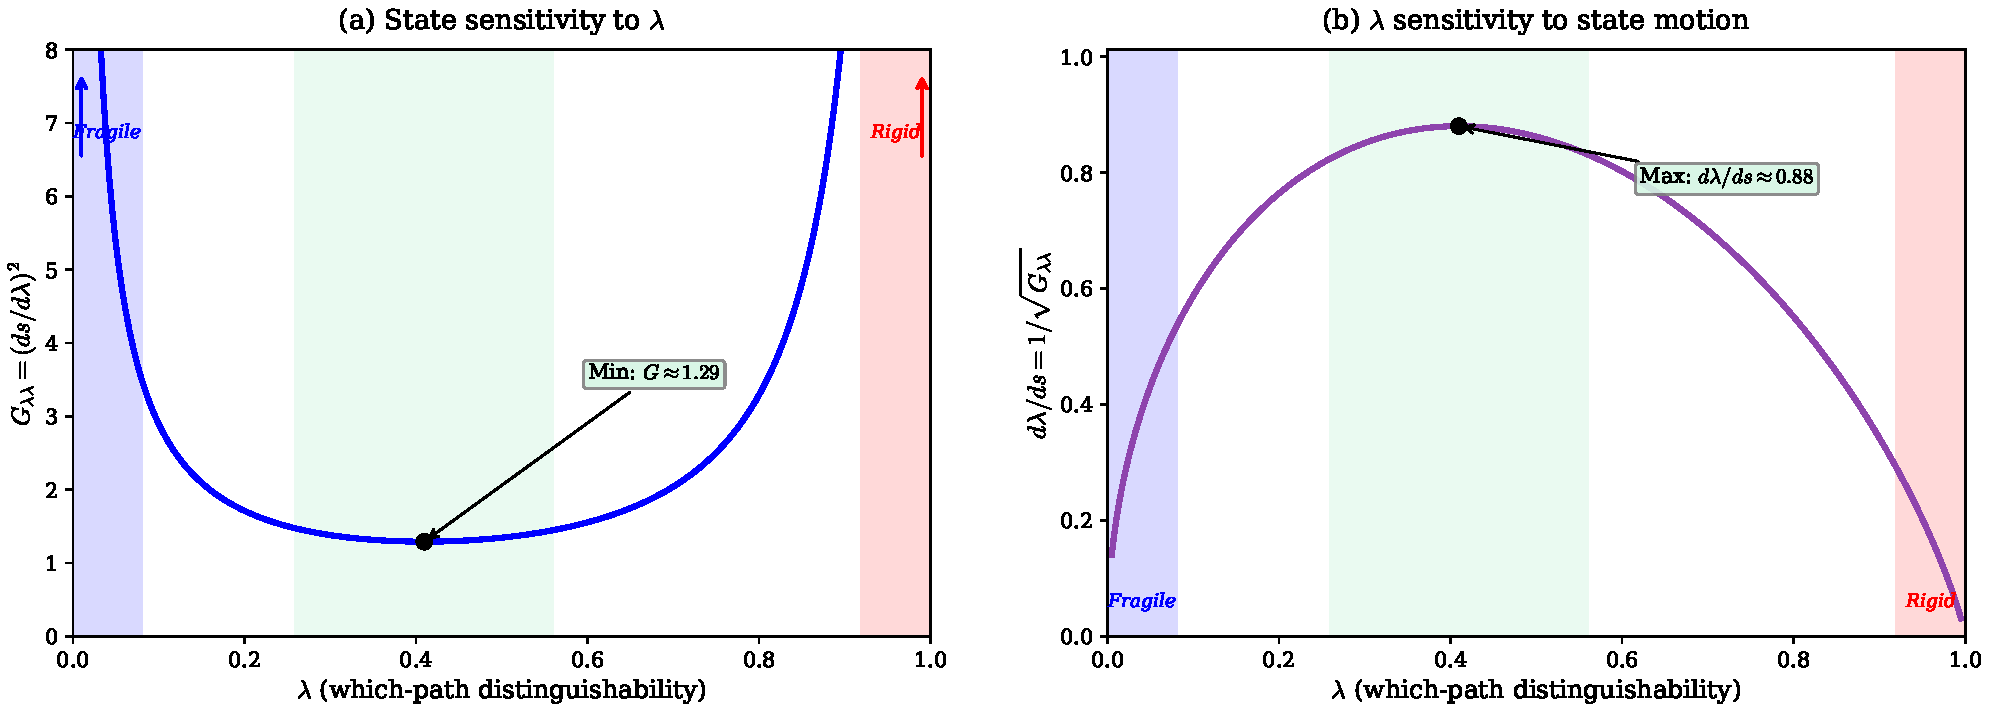
\includegraphics[width=\textwidth]{fig1_g_lambda.pdf}
\caption{Dual geometric views of the quantum--classical crossover (multi-mode decoherence, $N=10$). \textbf{(a)}~The Fubini--Study metric $\Gll = (ds/d\lambda)^2$ measures state sensitivity to distinguishability: large near both endpoints (geometric fragility of coherence, rigidity of classicality), minimal at $\lambda \approx 0.41$ (the crossover). \textbf{(b)}~The inverse $d\lambda/ds = 1/\sqrt{\Gll}$ measures how efficiently distinguishability grows per unit state motion: maximal at the crossover ($d\lambda/ds \approx 0.88$). Together, these identify the quantum--classical boundary as the region where the state resists change yet classical distinguishability emerges most efficiently.}
\label{fig:g_lambda}
\end{figure*}

\subsection{The Tensor Field $\Tab$}\label{sec:tensor}

The metric~\eqref{eq:fubini-study} captures the symmetric, information-geometric cost of moving between nearby frames. We now define the full tensor field $\Tab$ on~$\Sig$ that encodes both metric and connection structure.

\begin{definition}[Coherence Tensor Field]
Let $x^A$ denote local coordinates on~$\Sig$, with $A,B,\ldots$ indexing coherence-space directions. The \textbf{coherence tensor field} is
\begin{equation}\label{eq:tab-decomp}
\Tab(x) = G_{AB}(x) + \Omega_{AB}(x),
\end{equation}
where $G_{AB} = G_{BA}$ is symmetric and $\Omega_{AB} = -\Omega_{BA}$ is antisymmetric.
\end{definition}

\textbf{Symmetric part.} The metric $G_{AB}$ is the pullback of the Fubini--Study metric onto~$\Sig$ along the state map $x \mapsto \ket{\psi(x)}$:
\begin{equation}\label{eq:gab}
G_{AB}(x) = \mathrm{Re}\!\left[\braket{\partial_A \psi | \partial_B \psi} - \braket{\partial_A \psi | \psi}\!\braket{\psi | \partial_B \psi}\right],
\end{equation}
where $\partial_A := \partial/\partial x^A$. This is positive-semidefinite and measures the information-geometric cost of an infinitesimal frame change $\delta x^A$. Equation~\eqref{eq:fubini-study} is the one-dimensional restriction $\Gll = G_{AB}\,\delta^A_\lambda\,\delta^B_\lambda$ for the double-slit which-path parameter.

\textbf{Antisymmetric part.} The two-form $\Omega_{AB}$ derives from a connection $A_A$ on coherence space, with curvature $F_{AB} = \partial_A A_B - \partial_B A_A$. It encodes non-integrable aspects of frame changes: how coherence frames twist relative to each other along closed loops in~$\Sig$. In quasi-equilibrium situations (reversible frame changes), $\Omega_{AB} = 0$ and $\Tab$ reduces to the metric. For irreversible processes---such as partial erasure followed by attempted revival---$\Omega_{AB} \neq 0$ generates path-dependent (hysteretic) behavior.

\textbf{Double-slit reduction.} For the one-dimensional coherence manifold $\Sig \simeq [0,1]$ with which-path parameter~$\lambda$, the tensor field reduces to the single scalar component $T_{\lambda\lambda} = \Gll(\lambda)$ (since $\Omega_{\lambda\lambda} = 0$ trivially in one dimension). The full tensor structure becomes physically relevant for systems with $\dim\Sig \geq 2$, where closed loops in coherence space are possible.

The complete development of $\Tab$---including equations of motion, the quasipotential construction, and the connection to emergent spacetime---is the subject of Paper~2. Here we require only the decomposition~\eqref{eq:tab-decomp}, the metric definition~\eqref{eq:gab}, and the qualitative role of~$\Omega_{AB}$ in generating hysteresis.

\subsection{Analogy with Special Relativity}

The coherence-frame structure parallels the inertial-frame structure of special relativity (Table~\ref{tab:analogy}). The key structural parallel: in SR, there is no absolute simultaneity---it depends on the inertial frame. In \CR{}, there is no absolute fact about whether a system is ``in superposition'' or ``has collapsed''---it depends on the coherence frame.

\begin{table}[b]
\centering
\caption{Structural analogy between special relativity and coherence relativity.}\label{tab:analogy}
\begin{tabular}{@{}ll@{}}
\toprule
Special Relativity & Coherence Relativity \\
\midrule
Spacetime event & Physical reality $R$ \\
Inertial frame & Coherence frame $F$ \\
Coordinates $(t, \mathbf{x})$ & State representation $\ket{\psi}_F$ \\
Lorentz transformation & Frame transformation $U_{F \to F'}$ \\
Invariant interval $ds^2$ & Born measure $\mu = |c_i|^2$ \\
Minkowski metric & Fubini--Study metric on $\Sig$ \\
Simultaneity (relative) & Coherence (relative) \\
\bottomrule
\end{tabular}
\end{table}


% ============================================================
% SECTION 3: FRAME TRANSFORMATIONS
% ============================================================
\section{Frame Transformations and Invariants}\label{sec:transformations}

\subsection{Frame Transformation Maps}

\begin{definition}[Frame Transformation]
A \textbf{frame transformation} $U_{F \to F'}$ maps state representations: $\ket{\psi}_{F'} = U_{F \to F'}\ket{\psi}_F$. In the Hilbert space picture, $U_{F \to F'}$ is unitary:
\begin{equation}
\ket{i}_{F'} = \sum_j (U_{F \to F'})_{ji}\, \ket{j}_F.
\end{equation}
\end{definition}

\begin{definition}[Coherence Relabeling]
A \textbf{coherence relabeling} permutes and phase-rotates basis vectors:
\begin{equation}\label{eq:relabeling}
U_{F \to F'}: \ket{i}_F \to e^{i\theta_i}\ket{\pi(i)}_{F'},
\end{equation}
where $\pi$ is a permutation and $\theta_i \in \mathbb{R}$.
\end{definition}

\subsection{Group Structure}

Frame transformations form a \textbf{groupoid} over~$\Sig$:
\begin{enumerate}
\item Composition: $U_{F \to F''} = U_{F' \to F''} \circ U_{F \to F'}$
\item Identity: $U_{F \to F} = \mathbb{I}$
\item Inverse: $(U_{F \to F'})^{-1} = U_{F' \to F}$
\end{enumerate}
For finite-dimensional~$\mathcal{H}$, each $U_{F \to F'}$ has a unitary matrix representation preserving inner products: $\braket{\psi|\phi}_F = \braket{U\psi | U\phi}_{F'}$.

\subsection{Frame Splitting}\label{sec:splitting}

\begin{definition}[Frame Splitting]
A \textbf{frame splitting} transforms a single basis state into an equal-amplitude superposition:
\begin{equation}\label{eq:splitting}
\ket{i}_F \to \frac{1}{\sqrt{m_i}} \sum_{k=1}^{m_i} \ket{i,k}_{F'},
\end{equation}
where $\{\ket{i,k}_{F'}\}$ are orthonormal in the enlarged space.
\end{definition}

\begin{proposition}[Existence of Splittings]\label{prop:splitting}
For any state $\ket{\psi}_F = \sum_i c_i\ket{i}_F$ with rational $|c_i|^2 = m_i/M$ (where $M = \sum_i m_i$), there exists a splitting $F \to F'$ such that $\ket{\psi}_{F'} = M^{-1/2}\sum_{i,k}\ket{i,k}_{F'}$ is equal-amplitude.
\end{proposition}

\begin{proof}
Introduce an ancilla Hilbert space $\mathcal{H}_{\mathrm{anc}}$ of dimension~$M$ with orthonormal basis $\{\ket{e_j}\}_{j=1}^M$. Partition the ancilla basis into blocks: for each~$i$, assign $m_i$ ancilla states $\ket{e_{j}}$ with $j \in B_i$, where $|B_i| = m_i$ and the blocks are disjoint with $\bigcup_i B_i = \{1,\ldots,M\}$.

Define an isometry $V: \mathcal{H} \to \mathcal{H} \otimes \mathcal{H}_{\mathrm{anc}}$ by
\begin{equation}\label{eq:isometry}
V\ket{i}_F = \frac{1}{\sqrt{m_i}} \sum_{j \in B_i} \ket{i}_F \otimes \ket{e_j}.
\end{equation}
Then $V$ preserves inner products: $\bra{i}V^\dagger V\ket{i'} = \delta_{ii'}$. Applying $V$ to $\ket{\psi}_F$:
\begin{equation}
V\ket{\psi}_F = \sum_i c_i \cdot \frac{1}{\sqrt{m_i}} \sum_{j \in B_i} \ket{i,e_j} = \frac{1}{\sqrt{M}} \sum_{i}\sum_{j \in B_i} \ket{i,e_j},
\end{equation}
where the last equality uses $c_i = \sqrt{m_i/M}$ (up to phases absorbed by relabeling). Identifying $\ket{i,k}_{F'} \equiv \ket{i,e_j}$ for $j \in B_i$ gives the equal-amplitude state $\ket{\psi}_{F'} = M^{-1/2}\sum_{i,k}\ket{i,k}_{F'}$ in the enlarged frame~$F'$.
\end{proof}

Physically, this construction corresponds to refining a measurement by coupling to an ancilla---a standard procedure in quantum information.

\subsection{Frame Invariants}

\begin{theorem}[Frame Invariants]\label{thm:invariants}
The following are invariant under all frame transformations:
\begin{enumerate}
\item Total probability: $\sum_i \mu_F(i) = 1$
\item Born measures of alternatives: $\mu_F(i) = \mu_{F'}(\pi(i))$
\item Inner products: $|\!\braket{\psi|\phi}\!|^2$ is frame-independent
\item Eigenvalue spectra of observables
\item Entanglement entropy $S(\rho_A)$ for bipartite systems
\end{enumerate}
\end{theorem}

What is \emph{not} invariant: which observables have definite values, whether a state appears coherent or decohered, and the form of the density matrix.


% ============================================================
% SECTION 4: BORN RULE DERIVATION
% ============================================================
\section{The Born Rule as Frame-Invariant Measure}\label{sec:born}

The derivation that follows is Gleason-like in structure but replaces noncontextuality with frame-invariance: the symmetry is not ``the same observable measured by different projectors yields the same result'' but rather ``the same physical situation described in different coherence frames yields the same probabilities.''

\subsection{Statement}

The key symmetry underlying the derivation is invariance under refinement of alternatives. If two descriptions differ only by coupling to an ancilla that refines a single alternative into multiple orthogonal sub-alternatives of equal amplitude, then no physical probability assignment can distinguish between them. Such refinements are routine in quantum information and correspond operationally to increasing measurement resolution without altering the underlying physical situation. A probability measure that depended on whether or not such a refinement had been performed would be ill-defined, as it would assign different probabilities to physically equivalent descriptions. We formalize this requirement as invariance under frame splitting.

\begin{theorem}[Born Rule from Frame Invariance]\label{thm:born}
Let $\Sig$ be the coherence space for $\mathcal{H}$ with $\dim \geq 2$. Let $\mu$ be a measure on the alternatives $\{\ket{i}_F\}$ satisfying:
\begin{description}
\item[(A1)] \textbf{Frame invariance}: $\mu$ is invariant under coherence relabelings~\eqref{eq:relabeling} and frame splittings~\eqref{eq:splitting}.
\item[(A2)] \textbf{Additivity}: $\mu$ is additive on mutually orthogonal alternatives.
\item[(A3)] \textbf{Dependence}: $\mu_F(i)$ depends only on $\ket{\psi}_F$ and $\ket{i}_F$.
\item[(A4)] \textbf{Continuity}: $\mu_F(i)$ is continuous in the coefficients~$c_i$.
\end{description}
Then $\mu_F(i) = |c_i|^2$, where $\ket{\psi}_F = \sum_i c_i\ket{i}_F$.
\end{theorem}

\subsection{Derivation}

\textbf{Step 1: Phase independence.} By (A1), $\mu$ is invariant under coherence relabelings~\eqref{eq:relabeling}, including arbitrary phase rotations $\theta_i$. Hence $\mu_F(i)$ depends on $c_i$ only through $|c_i|$.

\textbf{Step 2: Equal amplitudes.} For $\ket{\psi}_F = N^{-1/2}\sum_{k=1}^N \ket{k}_F$, permutation invariance gives $\mu_F(k) = 1/N = |c_k|^2$ for all~$k$.

\textbf{Step 3: Rational amplitudes.} For $\ket{\psi}_F = \sqrt{m/(m+n)}\,\ket{0}_F + \sqrt{n/(m+n)}\,\ket{1}_F$, construct a frame splitting (Prop.~\ref{prop:splitting}) producing an equal-amplitude state of $m+n$ terms. By Step~2 and additivity~(A2):
\begin{equation}
\mu_F(0) = \frac{m}{m+n} = |c_0|^2, \quad \mu_F(1) = \frac{n}{m+n} = |c_1|^2.
\end{equation}

\textbf{Step 4: General amplitudes.} Approximate $|c_i|^2$ by rationals $r_i^{(n)}$ with $|r_i^{(n)} - |c_i|^2| < 1/n$. By Step~3, $\mu^{(n)}(i) = r_i^{(n)}$. By continuity~(A4), $\mu_F(i) = \lim_{n \to \infty} \mu^{(n)}(i) = |c_i|^2$.  \qed

\subsection{Comparison with Previous Derivations}

Table~\ref{tab:comparison} summarizes the relationship to prior work. The structural parallel with Zurek's envariance~\cite{zurekProbabilitiesEntanglementBorns2005} warrants explicit comparison. Both derivations use a splitting step to reduce general amplitudes to equal amplitudes. However, they differ in three respects: (i)~Zurek's envariance requires a physical environment and invokes swap symmetry of the system--environment state, which critics~\cite{zurekDecoherenceEinselectionQuantum2003} have argued presupposes the Born rule; our splitting (Prop.~\ref{prop:splitting}) is a mathematical theorem about Hilbert space embeddings, requiring no environment. (ii)~Envariance acts on a bipartite state $\ket{\psi}_{SE}$; frame invariance acts on the geometric structure of~$\Sig$ itself, making it independent of any particular physical setup. (iii)~The coherence-relativity derivation makes the \emph{geometric origin} of the symmetry manifest: frame invariance is the requirement that physics does not depend on which coherence frame is used for description, just as Lorentz invariance requires independence of inertial frame.

\begin{table*}[t]
\centering
\caption{Comparison of Born rule derivations.}\label{tab:comparison}
\begin{tabular}{@{}lllll@{}}
\toprule
Derivation & Symmetry Used & Physical Content & Assumes Born? & Result \\
\midrule
Gleason (1957) & Non-contextuality & Mathematical ($\mathcal{H}$) & No & $\mu = \mathrm{Tr}(\rho P)$ \\
Zurek (2005) & Envariance & Entanglement + environment & Debated & $\mu = |c_i|^2$ \\
Deutsch--Wallace & Rational equivalence & Many-worlds ontology & Debated & $\mu = |c_i|^2$ \\
Masanes et al.~\cite{masanesMeasurementPostulatesQuantum2019} & Operational axioms & Compositional structure & No & Born rule unique \\
\textbf{This work} & \textbf{Frame invariance} & \textbf{Geometric ($\Sig$, $\Tab$)} & \textbf{No} & $\boldsymbol{\mu = |c_i|^2}$ \\
\bottomrule
\end{tabular}
\end{table*}

\subsection{Physical Interpretation}

The Born rule is not a postulate, a frequency statement, or a consequence of branching. It is the \textbf{unique frame-invariant probability assignment} on~$\Sig$---the quantum analog of the invariant interval $ds^2$ in special relativity (Fig.~\ref{fig:born_invariant}).

\begin{figure}[t]
\centering
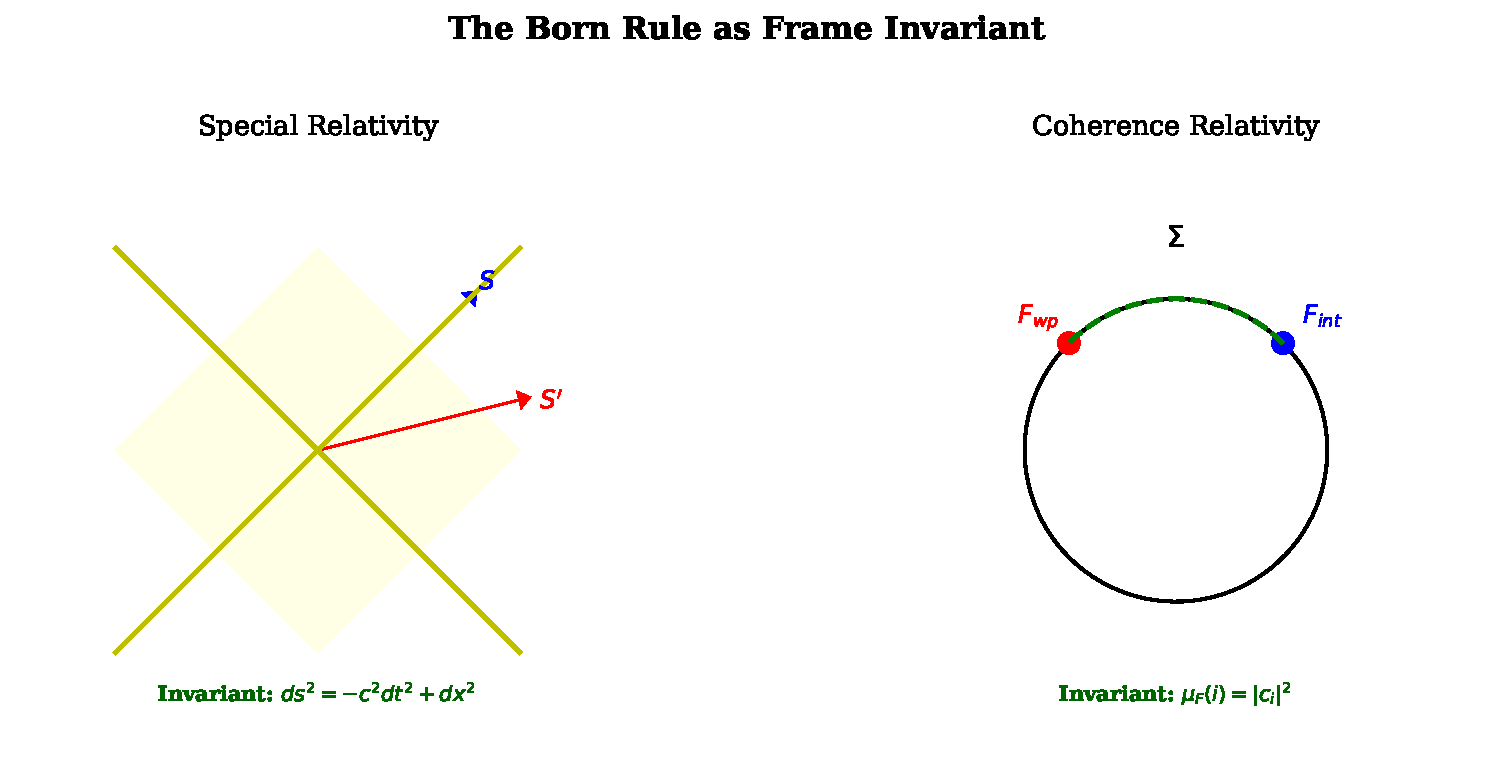
\includegraphics[width=\columnwidth]{fig4_born_rule_invariant.pdf}
\caption{The Born rule as frame invariant. Left: in special relativity, the interval $ds^2$ is invariant under Lorentz transformations. Right: in \CR{}, the Born measure $\mu_F(i) = |c_i|^2$ is invariant under coherence-frame transformations on~$\Sig$.}
\label{fig:born_invariant}
\end{figure}


% ============================================================
% SECTION 5: PARADOX RESOLUTIONS
% ============================================================
\section{Paradox Resolutions and Worked Examples}\label{sec:paradoxes}

\subsection{Double-Slit Experiment}

Consider the double-slit with two frames (Fig.~\ref{fig:double_slit}):
\begin{itemize}
\item $\Fint$: $\ket{\psi}_{\Fint} = \tfrac{1}{\sqrt{2}}(\ket{L} + \ket{R})$. Interference visible.
\item $\Fwp$: $\ket{\psi}_{\Fwp} = \tfrac{1}{\sqrt{2}}(\ket{L}\ket{W_L} + \ket{R}\ket{W_R})$. Paths definite.
\end{itemize}
The transformation $U_{\Fint \to \Fwp}$ is realized by detector coupling. Frame invariants: $\mu(L) = \mu(R) = 1/2$ in both frames. Frame-dependent: visibility of interference fringes, off-diagonal density matrix elements.

\begin{figure}[t]
\centering
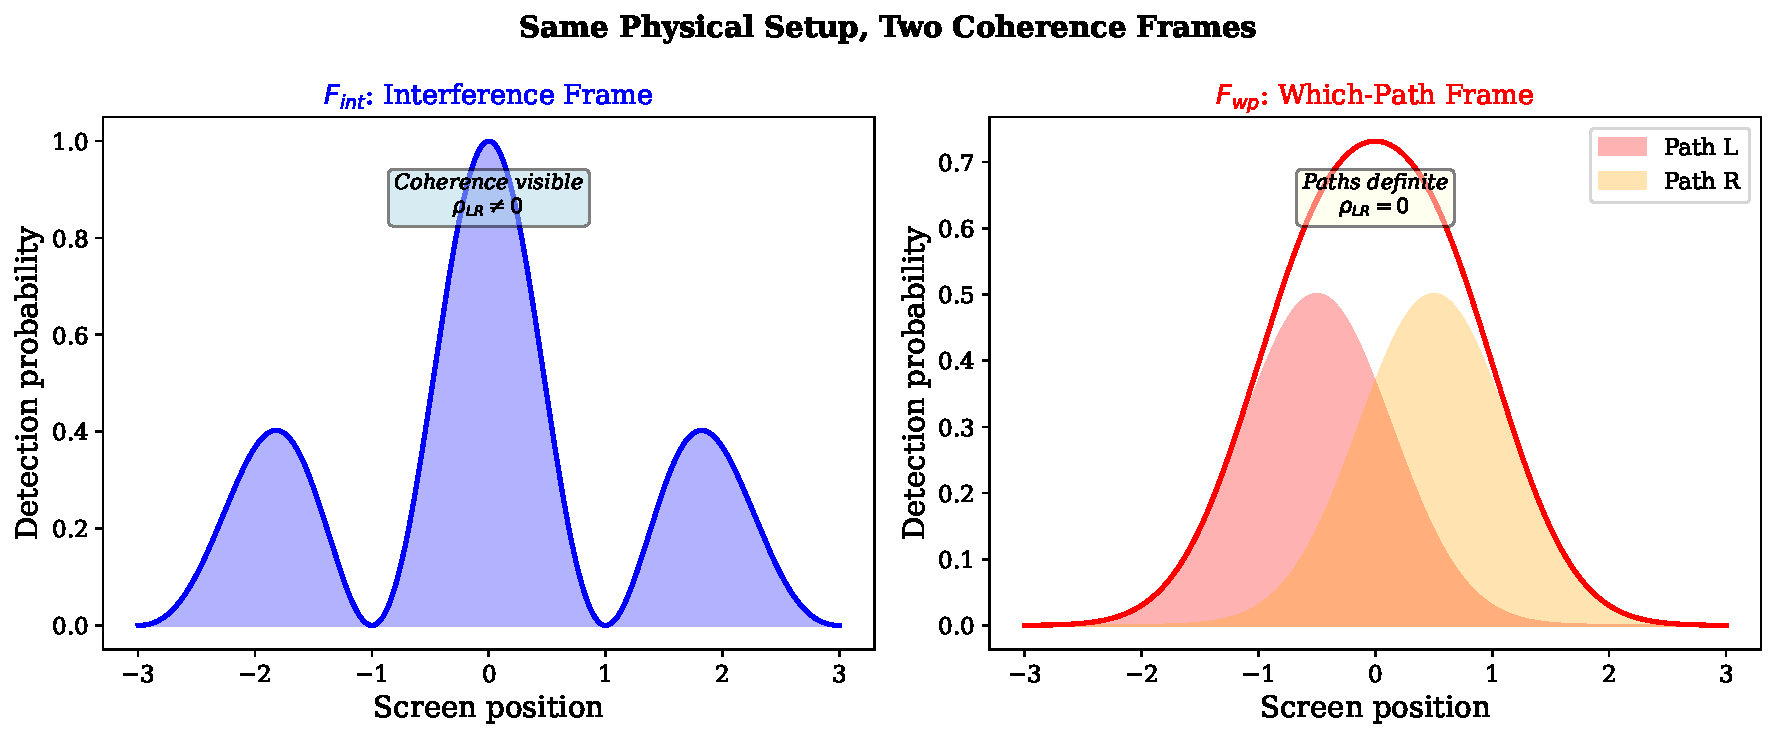
\includegraphics[width=\columnwidth]{fig5_double_slit_frames.pdf}
\caption{Double-slit experiment in two coherence frames. Left: interference frame~$\Fint$ shows the characteristic fringe pattern. Right: which-path frame~$\Fwp$ resolves individual paths with no interference. The Born measure $\mu(L) = \mu(R) = 1/2$ is invariant.}
\label{fig:double_slit}
\end{figure}

\subsection{Wigner's Friend}

Wigner's friend performs a measurement inside a laboratory (frame~$F_{\mathrm{friend}}$: state has collapsed to $\ket{\uparrow}$ or $\ket{\downarrow}$). Wigner, outside the lab, describes the joint system in $F_{\mathrm{Wigner}}$: the friend--system composite remains in superposition. In \CR{}, both descriptions are correct \emph{in their respective frames}. There is no contradiction, just as there is no contradiction between observers disagreeing about simultaneity in SR.

\subsection{EPR and Bell Nonlocality}

For an entangled pair in the singlet state, Alice's and Bob's local frames each see mixed states. The global frame sees entanglement. Bell inequality violation is a frame-invariant fact (it depends only on $|\!\braket{\psi|\phi}\!|^2$ terms). The correlations are not ``caused'' by collapse but are geometric properties of the entangled state visible from any frame.

\subsection{Schr\"odinger's Cat}

The cat-in-a-box scenario involves two frames: $F_{\mathrm{outside}}$ (cat in superposition) and $F_{\mathrm{inside}}$ (cat alive or dead). Opening the box is a frame transformation $U_{F_{\mathrm{outside}} \to F_{\mathrm{inside}}}$, not a physical collapse. The cat's definite state exists in $F_{\mathrm{inside}}$ at all times; it simply isn't accessible from $F_{\mathrm{outside}}$ without the frame transformation.


% ============================================================
% SECTION 6: DISCUSSION
% ============================================================
\section{Discussion}\label{sec:discussion}

\subsection{Resolution of the Measurement Problem}

\CR{} offers a relational resolution of the measurement problem: ``collapse'' is a frame transformation, not a dynamical process. The Born rule is not postulated but derived as the unique frame-invariant measure. Definite outcomes exist in appropriate coherence frames; superposition exists in others. There is no need to explain \emph{when} or \emph{how} collapse occurs, because collapse is not a physical event---it is a change of description. Crucially, no frame ever loses coherence: what changes is the geometric relationship between alternatives, as distinguishability becomes redundantly encoded in the environment. Coherence is not destroyed but \emph{re-described} from the perspective of a different frame.

\subsection{Quasipotential Landscape}

The tensor field~$\Tab$ (Sec.~\ref{sec:tensor}) generates a quasipotential landscape on~$\Sig$ via an action principle. For a path $\gamma: s \mapsto x(s)$ through coherence space with effective drift~$F^A(x)$ (driven by system--environment coupling) and noise scale~$D$, define the action
\begin{equation}\label{eq:action}
\mathcal{S}[\gamma] = \frac{1}{4D}\int_0^1 (\dot{x}^A - F^A)\,G_{AB}\,(\dot{x}^B - F^B)\,ds.
\end{equation}
The quasipotential is $V(x) = \inf_\gamma \mathcal{S}[\gamma]$, where the infimum is over paths from a reference frame to~$x$ (Fig.~\ref{fig:quasipotential}). Minima of~$V$ correspond to metastable classical frames (pointer states), saddle points determine transition rates, and the stationary distribution concentrates as $p(x) \propto \exp(-V(x)/\epsilon)$ for small effective noise~$\epsilon$. This provides a geometric explanation for einselection: environment-induced superselection is the dynamical relaxation to $V$-minima.

The accumulated Fubini--Study length $s(\lambda) = \int_0^\lambda\!\sqrt{\Gll}\,d\lambda'$ reveals a \emph{geometric activation distance} $s^* \equiv s(\lambda^*)$, where $\lambda^*$ is the crossover point at which $d\lambda/ds$ is maximal (Fig.~\ref{fig:g_lambda}b). For the multi-mode model ($N=10$), $s^* \approx 0.72$: the state must traverse this minimum Fubini--Study length before distinguishability can grow efficiently. The crossover plateau in $s(\lambda)$---where $\lambda$ increases substantially while $s$ changes little---is analogous to latent heat in a first-order phase transition: the system absorbs geometric ``work'' (environment entanglement) without proportionate change in the macroscopic order parameter. This analogy is exact in the sense that both phenomena reflect a flat region of the relevant potential landscape separating two steep walls.

\begin{figure}[t]
\centering
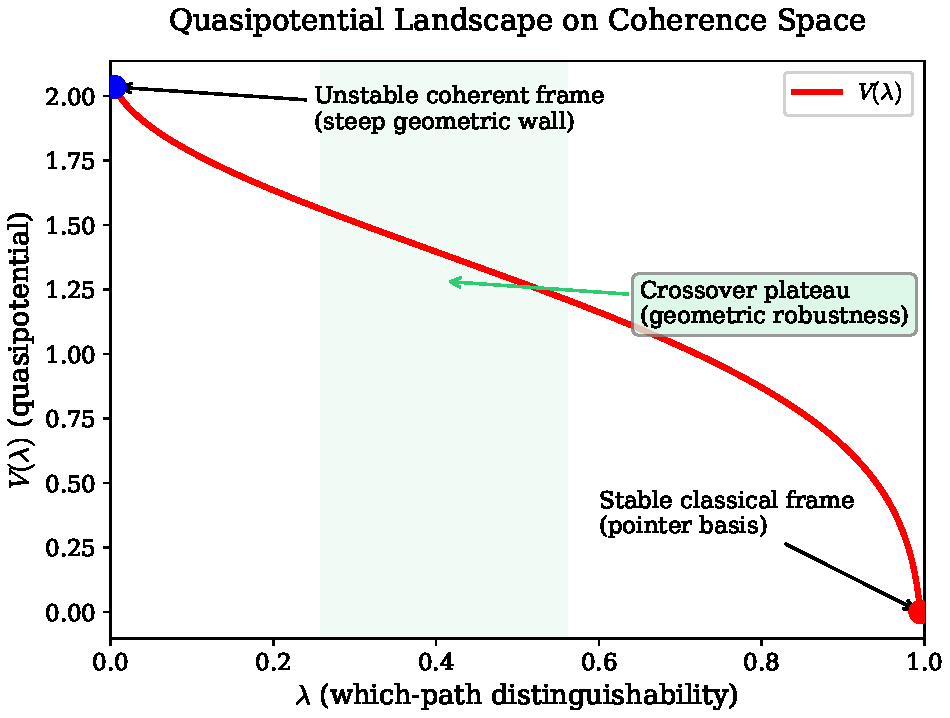
\includegraphics[width=\columnwidth]{fig2_quasipotential.pdf}
\caption{Quasipotential $V(\lambda) = \int_\lambda^1 \!\sqrt{\Gll}\,d\lambda'$ on coherence space, measuring the accumulated Fubini--Study distance to the classical frame. The steep walls at both endpoints reflect the divergent metric (geometric fragility of coherence, rigidity of classicality), while the gentle intermediate slope identifies a crossover plateau where large increases in distinguishability produce only small movements in projective Hilbert space. The global minimum at $\lambda = 1$ (pointer basis) represents the stable classical frame.}
\label{fig:quasipotential}
\end{figure}

\subsection{Quantum Darwinism and Objectivity}

\CR{} naturally accommodates quantum Darwinism~\cite{zurekQuantumDarwinism2009}: when multiple environment fragments independently acquire the same information about the system, they select a preferred coherence frame. In \CR{} language, the redundant encoding of pointer-state information across environment fragments~\cite{riedelObjectiveQuantumUniverse2016,korbiczObjectivityNoisyPhotonic2017} corresponds to the narrowing of the quasipotential well around the classical frame as the number of monitoring fragments~$N$ increases.

\subsection{Testable Predictions}

Six experimentally testable signatures distinguish \CR{} from standard QM:
\begin{enumerate}
\item \textbf{Non-linear visibility}: $\mathcal{V}(\lambda)$ deviates from $\sqrt{1-\lambda^2}$ due to $\Gll$ curvature (Fig.~\ref{fig:cr_vs_standard}).
\item \textbf{Frame-transformation hysteresis}: Erasure paths $\lambda: 0 \to 1 \to 0$ show path-dependent visibility recovery.
\item \textbf{Coherence-space curvature}: Many-body systems exhibit $\Gll$ scaling deviations from mean-field predictions.
\item \textbf{Modified gravitational decoherence}: Gravitational contributions to~$\Tab$ produce mass-dependent frame-transformation rates differing from Di\'osi--Penrose~\cite{diosiUniversalMasterEquation1987,penroseGravitysRoleQuantum1996}.
\item \textbf{Transformation timescales}: Weak measurements probe finite frame-transformation duration, resolvable with current qubit platforms.
\item \textbf{Coherence revival}: Closed systems show partial coherence recovery forbidden in irreversible-collapse models~\cite{ghirardiUnifiedDynamicsMicroscopic1986,carlessoTestingLargescaleLimit2020}.
\end{enumerate}

\begin{figure}[t]
\centering
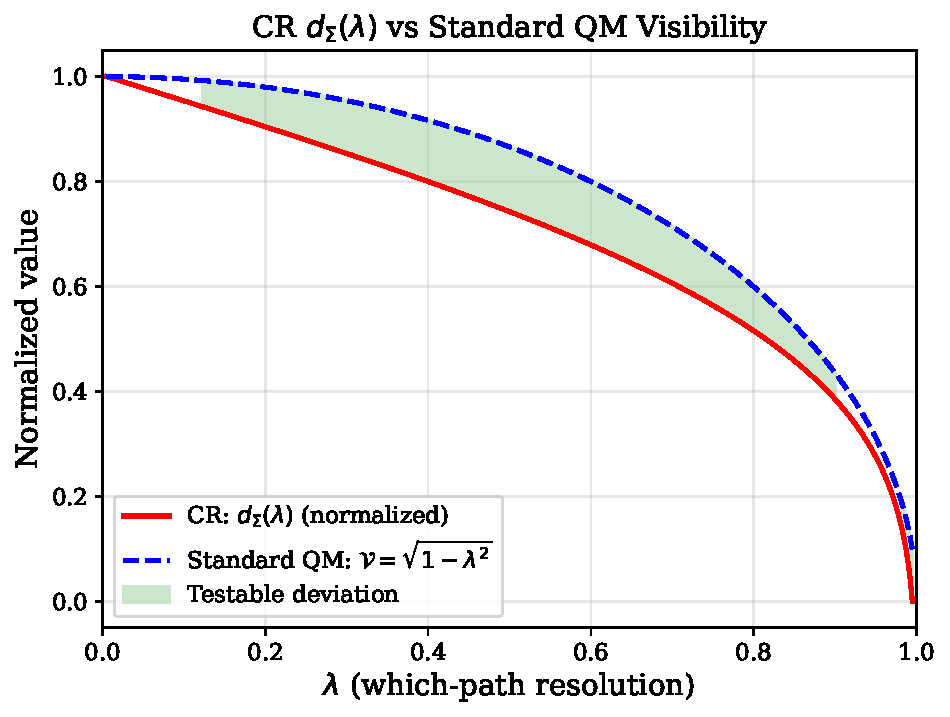
\includegraphics[width=\columnwidth]{fig6_cr_vs_standard.pdf}
\caption{Comparison of the normalized \CR{} geometric transition $V(\lambda)/V(0)$ (solid, red) with standard QM visibility $\mathcal{V} = \sqrt{1-\lambda^2}$ (dashed, blue). The CR curve drops faster through the crossover region due to the metric structure, producing a testable deviation $\Delta \approx 0.24$ at intermediate~$\lambda$.}
\label{fig:cr_vs_standard}
\end{figure}

\subsubsection{Quantitative estimates}

We provide order-of-magnitude estimates for the two most accessible predictions.

\textit{Frame-transformation hysteresis.} Consider a qubit coupled dispersively to a readout resonator (dispersive shift $\chi/2\pi \sim 1$~MHz). Prepare the state $\ket{+} = (\ket{0}+\ket{1})/\sqrt{2}$, drive the which-path parameter through a cycle $\lambda: 0 \to \lambda_{\max} \to 0$ by pulsing the readout, then measure visibility. In standard QM with a closed erasure cycle, $\mathcal{V}_{\mathrm{revival}} = \mathcal{V}_{\mathrm{initial}}$. In \CR{}, the action cost of the cycle is
\begin{equation}\label{eq:hysteresis}
\Delta\mathcal{S} = \frac{1}{4D}\oint (\dot\lambda - F^\lambda)^2 \Gll\,ds > 0,
\end{equation}
yielding a visibility deficit $\delta\mathcal{V} \sim (\tau_{\mathrm{frame}}/T_2)^2 \cdot \mathcal{R}_\Sig$, where $\tau_{\mathrm{frame}} \sim 1/\chi \approx 1\;\mu$s is the frame-transformation timescale, $T_2 \approx 70\;\mu$s is the dephasing time, and $\mathcal{R}_\Sig = 8$ is the Ricci scalar of the qubit coherence space ($\mathrm{CP}^1$ with the Fubini--Study metric has radius $1/2$, giving $\mathcal{R} = 2/r^2 = 8$). This gives $\delta\mathcal{V} \sim 2 \times 10^{-3}$---small but within the sensitivity of current superconducting qubit tomography ($\sim 10^{-3}$ with $\sim 10^5$ repetitions).

\textit{Transformation timescales.} The geodesic distance in~$\Sig$ between the coherent frame ($\lambda = 0$) and the pointer frame ($\lambda = 1$) sets a minimum transformation duration:
\begin{equation}\label{eq:tau}
\tau_{\mathrm{frame}} = \frac{1}{v_{\max}}\int_0^1 \sqrt{\Gll(\lambda)}\,d\lambda,
\end{equation}
where $v_{\max}$ is bounded by the measurement coupling strength. For a transmon qubit with $\chi/2\pi = 1$~MHz coupled to a single readout resonator ($N=1$), the metric takes the form $\Gll = 1/[2\lambda(2-\lambda)]$ and the geodesic integral evaluates analytically to $\int_0^1\!\sqrt{\Gll}\,d\lambda = \pi/(2\sqrt{2}) \approx 1.1$, giving $\tau_{\mathrm{frame}} \gtrsim 1.1\;\mu$s. For multi-mode environments ($N=10$, Fig.~\ref{fig:g_lambda}), the integral over the experimentally accessible range ($\lambda \in [0.01, 0.99]$, excluding the coordinate-singular endpoints) evaluates to $\approx 2.0$. Both timescales are resolvable via weak-measurement trajectories~\cite{carlessoTestingLargescaleLimit2020}: monitoring the qubit with a weak probe during the frame transformation should reveal a finite-duration transition rather than an instantaneous jump, with the transition profile reflecting the characteristic U-shaped $\Gll(\lambda)$ from Fig.~\ref{fig:g_lambda}. Since the physical decoherence rate satisfies $ds/dt = \sqrt{\Gll}\,d\lambda/dt$, the metric directly shapes the temporal trajectory: rapid state evolution near the endpoints (where $\Gll$ diverges) and slow passage through the crossover (where $\Gll$ is minimal).

\medskip
\noindent\fbox{\parbox{\columnwidth-2\fboxsep-2\fboxrule}{\small\textbf{Remark on universality.} The timescales above are \emph{not} universal predictions of the framework: they depend on the coupling strength~$v_{\max}$ that sets the maximum rate of motion through~$\Sig$. What \emph{is} universal is the geometric constraint~\eqref{eq:tau}---a minimum geodesic distance must be traversed---and the characteristic shape of~$\Gll(\lambda)$. Different experimental platforms (femtosecond photonic vs.\ microsecond superconducting) will exhibit different absolute timescales because their couplings differ; the testable content is the \emph{ratio} of transformation duration to coupling strength and the path-dependent structure of the metric.}}
\medskip
\subsection{Relationship to Existing Frameworks}

\CR{} is closest in spirit to relational quantum mechanics~\cite{rovelliRelationalQuantumMechanics1996} but differs in three respects: (i)~$\Sig$ has concrete geometric structure; (ii)~the Born rule is derived, not assumed; (iii)~the tensor field~$\Tab$ provides dynamics absent in RQM.

Compared to QBism~\cite{fuchsIntroductionQBism2014}, \CR{} is realist: frame-invariant content (Born measures, inner products, spectra) constitutes observer-independent physical fact.

Compared to many-worlds~\cite{everettRelativeStateFormulation1957,dewittManyWorldsInterpretationQuantum1973}, \CR{} posits one reality and many frames, not many worlds and one agent. The logical structure of the Born rule derivation parallels the Deutsch--Wallace approach, but replaces branching ontology with geometric frame-invariance.

The quantum reference frame (QRF) program~\cite{bartlettReferenceFramesSuperselection2007,giacominiQuantumMechanicsCovariance2019,delahametteQuantumReferenceFrames2020} shares \CR{}'s emphasis on frame-dependence: Giacomini et al.\ showed that entanglement and superposition are QRF-dependent~\cite{giacominiQuantumMechanicsCovariance2019}, and perspective-neutral approaches~\cite{vanrietveldeChangePerspectiveSwitching2020,loveridgeSymmetryReferenceFrames2018} seek frame-invariant structures. \CR{} differs in scope: QRFs transform between quantum systems serving as references, while coherence frames transform between \emph{descriptive bases} for a fixed system. The coherence space~$\Sig$ provides a global geometric arena absent in QRF treatments, and the Born rule emerges as its unique invariant measure rather than being assumed. Recent work showing that the sum of entanglement and subsystem coherence is invariant under QRF transformations~\cite{cepollaroSumEntanglementSubsystem2025} provides independent support for the principle that frame-invariant quantities---not frame-dependent descriptions---constitute physical reality. Figure~\ref{fig:sigma-qrf} summarizes the structural distinction.

\medskip
\noindent\textbf{Minimal ontology.} To summarize the interpretive commitments: \CR{} posits \emph{one reality~$R$}, \emph{many coherence frames~$F \in \Sig$}, and \emph{frame-invariant quantities as physical facts}. Collapse, coherence, and classicality are frame-dependent descriptions; Born measures, inner products, spectra, and entanglement entropy are frame-invariant and constitute observer-independent reality.
\medskip
\begin{figure*}[t]
\centering
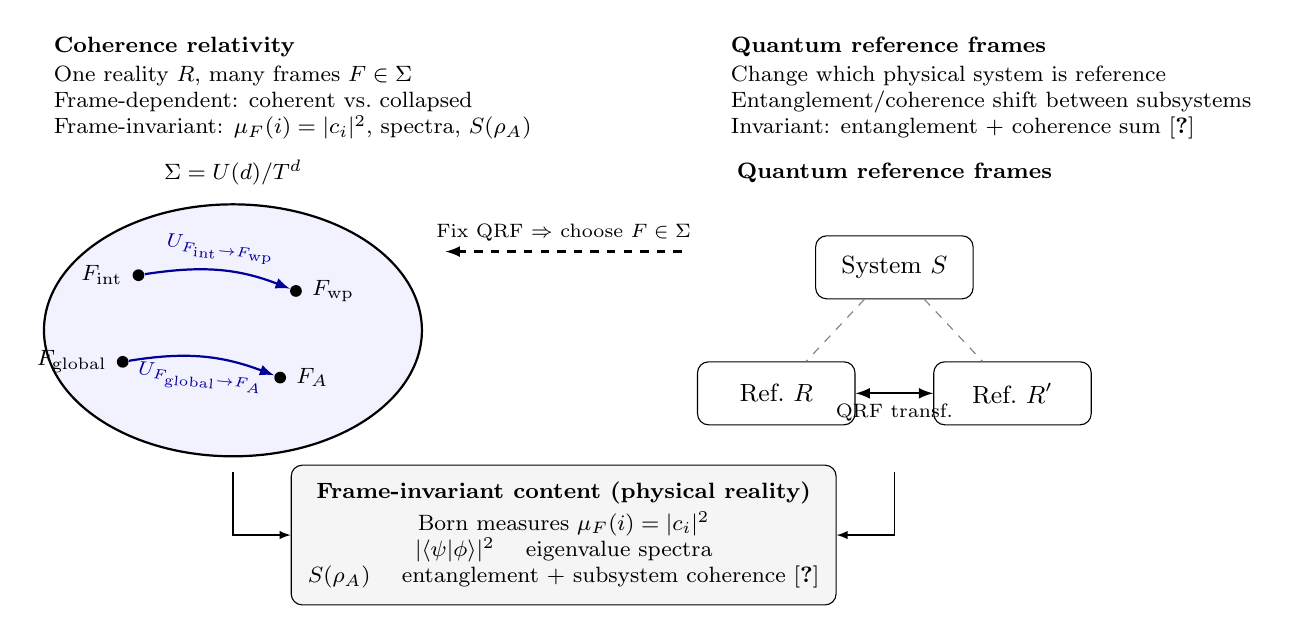
\begin{tikzpicture}[
  >=latex,
  every node/.style={font=\small},
  descbox/.style={align=left,font=\footnotesize,anchor=south west},
  panellabel/.style={font=\footnotesize\bfseries},
  framedot/.style={circle,fill=black,inner sep=1.5pt}
]
%
% --- Top row: CR and QRF descriptions (above the diagrams) ---
\node[descbox] at (-6.6,2.3) {%
  \textbf{Coherence relativity}\\[1pt]
  One reality $R$, many frames $F\in\Sig$\\
  Frame-dependent: coherent vs.\ collapsed\\
  Frame-invariant: $\mu_F(i)=|c_i|^2$, spectra, $S(\rho_A)$};
\node[descbox] at (2.0,2.3) {%
  \textbf{Quantum reference frames}\\[1pt]
  Change which physical system is reference\\
  Entanglement/coherence shift between subsystems\\
  Invariant: entanglement + coherence sum~\cite{cepollaroSumEntanglementSubsystem2025}};
%
% --- Left panel: coherence manifold Sigma ---
\begin{scope}[shift={(-4.2,0)}]
  % Smooth blob for the manifold
  \draw[thick,fill=blue!5]
    (0,0) ellipse [x radius=2.4cm, y radius=1.6cm];
  \node[panellabel] at (0,2.0) {$\Sig = U(d)/T^d$};
  % Frame points
  \node[framedot,label={[font=\footnotesize]left:$\Fint$}] (Fint) at (-1.2,0.7) {};
  \node[framedot,label={[font=\footnotesize]right:$\Fwp$}] (Fwp) at (0.8,0.5) {};
  \node[framedot,label={[font=\footnotesize]left:$F_{\mathrm{global}}$}] (Fglob) at (-1.4,-0.4) {};
  \node[framedot,label={[font=\footnotesize]right:$F_A$}] (FA) at (0.6,-0.6) {};
  % Transformation arrows
  \draw[->,thick,blue!60!black] (Fint) to[bend left=15]
    node[above,sloped,font=\scriptsize]{$U_{\Fint\to\Fwp}$} (Fwp);
  \draw[->,thick,blue!60!black] (Fglob) to[bend left=15]
    node[below,sloped,font=\scriptsize]{$U_{F_{\mathrm{global}}\to F_A}$} (FA);
\end{scope}
%
% --- Right panel: QRFs ---
\begin{scope}[shift={(4.2,0)}]
  \node[panellabel] at (0,2.0) {Quantum reference frames};
  \node[draw,rounded corners,minimum width=2cm,minimum height=0.8cm,fill=white] (S) at (0,0.8) {System $S$};
  \node[draw,rounded corners,minimum width=2cm,minimum height=0.8cm,fill=white] (R) at (-1.5,-0.8) {Ref.\ $R$};
  \node[draw,rounded corners,minimum width=2cm,minimum height=0.8cm,fill=white] (Rp) at (1.5,-0.8) {Ref.\ $R'$};
  \draw[<->,thick] (R) -- node[below,font=\scriptsize]{QRF transf.} (Rp);
  \draw[-,dashed,gray] (S) -- (R);
  \draw[-,dashed,gray] (S) -- (Rp);
\end{scope}
%
% --- Mapping arrow ---
\draw[dashed,->,thick] (1.5,1.0) -- node[above,font=\scriptsize]{Fix QRF $\Rightarrow$ choose $F\in\Sig$} (-1.5,1.0);
%
% --- Bottom inset: frame-invariant content (4 lines, narrowed) ---
\node[draw,rounded corners,align=center,fill=gray!8,inner sep=6pt,font=\footnotesize] (inv) at (0,-2.6) {%
  \textbf{Frame-invariant content (physical reality)}\\[2pt]
  Born measures $\mu_F(i) = |c_i|^2$\\
  $|\!\braket{\psi|\phi}\!|^2$ \quad eigenvalue spectra\\
  $S(\rho_A)$ \quad entanglement + subsystem coherence~\cite{cepollaroSumEntanglementSubsystem2025}};
% Arrows point to the outside (left and right) of the box
\draw[->] (-4.2,-1.8) |- (inv.west);
\draw[->] (4.2,-1.8) |- (inv.east);
\end{tikzpicture}
\caption{Coherence relativity vs.\ quantum reference frames. Left: the coherence manifold $\Sig$ with frames $F$ connected by transformations $U_{F\to F'}$. Coherence and collapse are frame-dependent; Born measures and spectra are invariant. Right: QRF transformations change which physical system serves as reference, redistributing entanglement and coherence between subsystems. Dashed arrow: given any QRF choice, one still selects a coherence frame $F \in \Sig$ on the resulting Hilbert space. Bottom: physical reality consists of quantities invariant under both types of transformation.}
\label{fig:sigma-qrf}
\end{figure*}


% ============================================================
% SECTION 7: CONCLUSION
% ============================================================
\section{Conclusion}\label{sec:conclusion}

We have introduced coherence relativity, a geometric framework in which:
\begin{enumerate}
\item Quantum coherence is frame-relative, like simultaneity in special relativity.
\item The Born rule $\mu_F(i) = |c_i|^2$ is the unique frame-invariant probability measure on the coherence manifold~$\Sig$.
\item Wave function collapse is a frame transformation, not a dynamical process.
\item The information geometry of~$\Sig$, encoded in the Fubini--Study metric and the tensor field~$\Tab$, generates a quasipotential landscape explaining einselection and classical emergence.
\end{enumerate}

The framework unifies insights from Gleason, Zurek, and operational reconstruction programs while identifying six experimentally testable signatures. The most accessible---frame-transformation hysteresis and measurable transformation timescales---are within reach of current superconducting qubit and trapped ion experiments.

\pagebreak

Paper~2 will develop the full tensor field~$\Tab$ on $\mathcal{M} \times \Sig$, derive the equations of motion for frame dynamics, and explore holographic connections between coherence-space geometry and emergent spacetime.

% ============================================================
% DECLARATIONS (Required by Foundations of Physics)
% ============================================================
\section*{Declarations}

\subsection*{Competing Interests}
The author declares no competing financial or non-financial interests.

\subsection*{Data Availability Statement}
All numerical data supporting the results in this study (Fubini--Study metric calculations, quasipotential landscapes, and figure generation) are available from the author upon reasonable request. The Python scripts used to generate these data are openly available at \url{https://github.com/bryankaufman/coherence-relativity}. No experimental datasets were generated or analyzed in this theoretical study.

\subsection*{Funding}
This work received no specific grant from any funding agency in the public, commercial, or not-for-profit sectors.

\subsection*{Author Contributions}
B.K. conceived the theoretical framework, performed all calculations, generated all figures, and wrote the manuscript.

\onecolumngrid
\begin{acknowledgments}
The author thanks the members of the Society of Mind coordination network for research assistance and computational support. The author is grateful to the open-source scientific Python community for tools enabling the numerical calculations presented herein.
\end{acknowledgments}
\twocolumngrid

\bibliography{../../bibliography/master}

\end{document}
